\section{Problem formulation}
\label{sec:cod_problem}
As outlined in previous chapters, the primary objective of this thesis is to validate the possibility of using object priors to enhance the system ability to ignore distractor objects during task execution, while simultaneously providing human-readable information about the robot behavior.

In Section \ref{sec:ooil}, various methods that utilize object priors in the context of Imitation Learning have been discussed. However, all the methods described in that section rely on pre-trained object detectors to identify regions of interest, i.e., areas that potentially contain objects, regardless of the object class (e.g., box, nut, bin, peg, etc.) or its semantic state (i.e., whether the object is relevant to the task or merely a distractor). Furthermore, none of these methods are designed for multi-variation scenarios, where the semantic state of an object (whether it is relevant or a distractor) is dynamically determined by the requirements of the specific task.

In the context of interest, the object detection problem can be formulated as follows: given a pair consisting of an agent observation and a command, $\left( o_{t}^{a}, c_{m_{i}} \right)$,  a parameterized function $f_{\theta}$, must generate a set of bounding boxes (bb), $\left\{ bb^{j}_{t} | j \in C \right\}$ that identifies \textbf{specific} regions of interest, i.e., $\left\{ bb^{j}_{t} | j \in C \right\} = f_{\theta}(o_{t}^{a}, c_{m_{i}})$. Here, $C$ represents a set of classes assigned to the bounding boxes, which differs from the traditional object detection classes. Instead of predicting the object category (e.g., box, nut, bin, etc.), the focus is on predicting the \textbf{semantic attribute} associated with each object. In the most general case, these attributes are:

\begin{itemize} 
    \item \textit{Target}, it indicates that the bounding box refers to the object to be manipulated in the current task variation $c_{m_{i}}$. 
    \item \textit{No-Target}, it refers to any other object in the scene that is not being manipulated. 
    \item \textit{Target-Place}, it represents the final region of interest for the manipulated object, which varies depending on the task. For example, in a pick-and-place task, it refers to the bin where the object is placed; in a nut-assembly task, it refers to the peg where the object is inserted; and in a button-press task, it refers to the region where the button has been pressed. 
    \item \textit{No-Target-Place}, it refers to any other region that is not relevant to the current task variation, such as other bins in a pick-and-place task or other pegs in a nut-assembly task. 
\end{itemize}

This example highlights how the semantic attribute assigned to an object changes depending on the requested task $c_{m}$. In the first case, the green box and the first bin are marked as targets (green boxes), while other objects are labeled as distractors (red boxes). In the second case, even though the configuration remains the same, the roles of the objects changes. This is because, in the second task, the demonstrator manipulates the red box and places it into a different location. 

Since the goal is to explicitly manage the changing semantic meaning of objects, traditional object detectors, which predict bounding boxes and object categories for all objects in the scene, are not suitable. Instead, a novel, specialized architecture is required to implement the function $f_{\theta}$. The details of this implementation are provided in Section \ref{sec:cod_architecture}.
\begin{figure}[t]
    \centering
    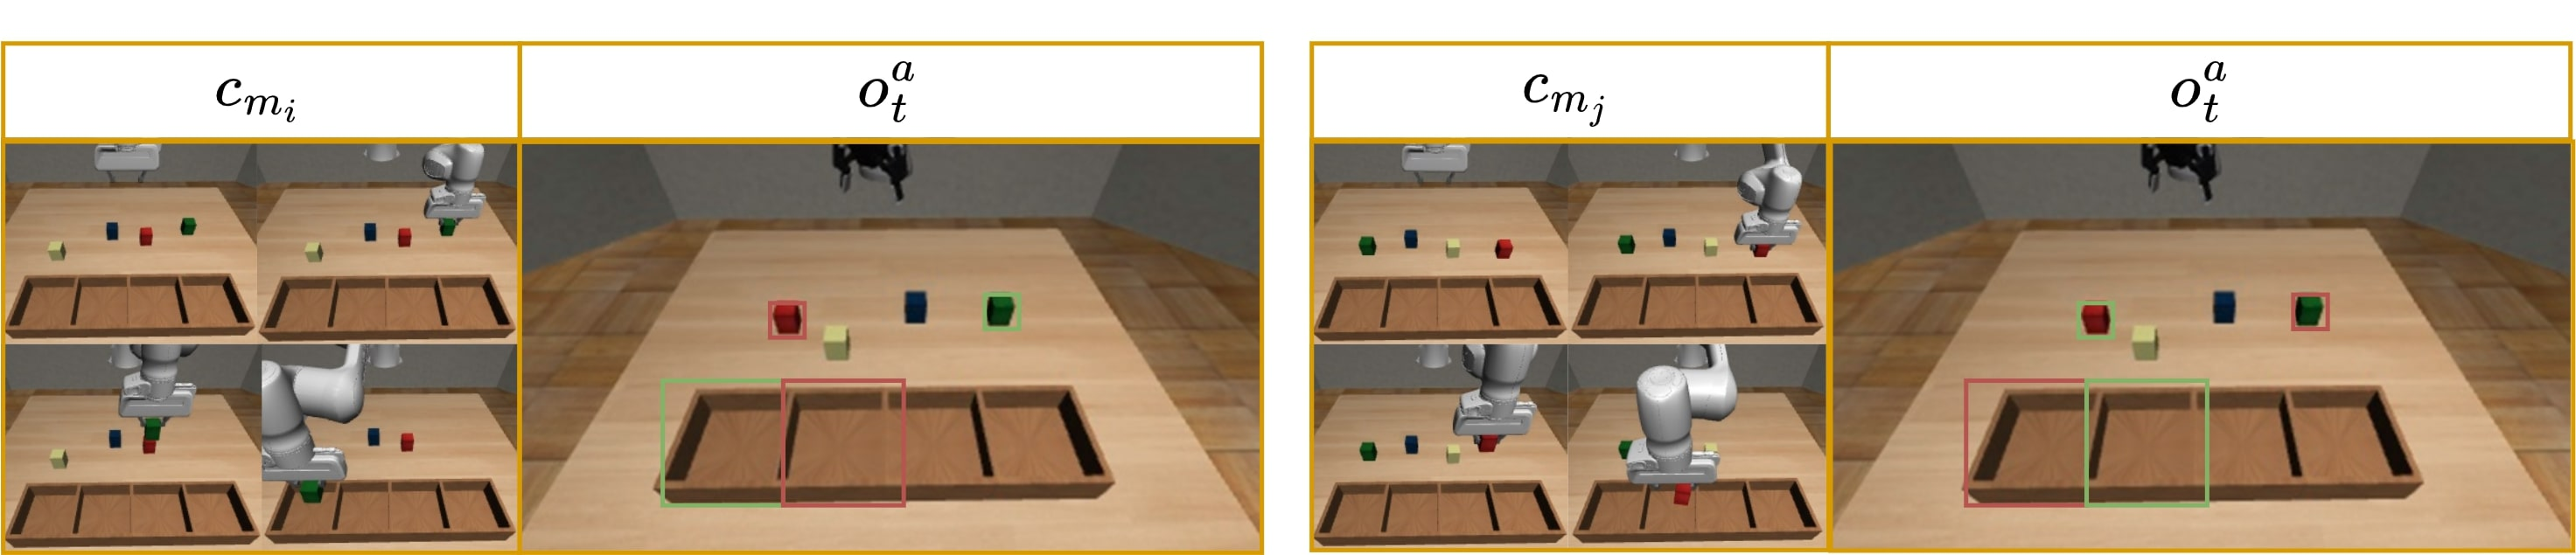
\includegraphics[width=1.0\textwidth]{figures/images/ch2/example_of_bb.jpg}
    \caption{Example of bounding-boxes assignment, where green boxes refer to target object and placing location while red boxed refers to no-target and no-target-place. (Left) The demonstrator manipulates the green box, placing it into the first bin. (Right) The demonstrator manipulates the red box, placing it into the second bin. Note, how for a given agent environment state, the semantic attribute between objects changes.}
    \label{fig:example_of_bb}
\end{figure}



